\documentclass{article}
\usepackage[utf8]{inputenc}
\usepackage[margin=1in,includefooter]{geometry}
\usepackage{graphicx}
\usepackage{float}

\begin{document}

\begin{titlepage}
    \begin{center}
    \line(1,0){300} \\
    [0.2in]
    \huge{\bfseries Knapsack Problem\\ Comparison Report} \\
    \line(1,0){300} \\
    [1.5cm]
    \textsc{\LARGE Greedy vs. Dynamic vs. Exhaustive}\\
    [15cm]
    \end{center}
    \begin{flushright}
    \textsc{\large Samy Masadi\\
    CSCI 423\\
    April 12, 2019}
    \end{flushright}
\end{titlepage}

\tableofcontents
\thispagestyle{empty}
\cleardoublepage

\setcounter{page}{1}

\section{Summary}
\hspace{\parindent}The program knapsack\_problem.py demonstrates and measures the performance of three different solutions to the 0-1 knapsack problem. The greedy ratio algorithm selects the best value/weight ratio item one at a time until the knapsack is filled. The dynamic programming algorithm determines the best value for a capacity and items available by building on previously calculated values that it has stored in memory. The exhaustive search is a brute force algorithm that iterates through every possible combination of items and keeps track of which both fits in the knapsack and has the highest value.

Both dynamic programming and exhaustive search produce the most optimal value combination of items, while the greedy ratio will not always be optimal. The exhaustive search is always optimal because it checks every combination. Dynamic programming considers whether each item will produce an optimal combination by comparing the value with its inclusion to the previously saved best value without its inclusion. The greedy method, meanwhile, is only concerned with the best ratio item at the time. Since it does not consider the whole combination, it will sometimes ignore items simply because they do not have the best ratio at the time of selection.

As far as time and space efficiency, the greedy and dynamic algorithms are much better than the exhaustive search. With any n and capacity beyond small values, brute force becomes prohibitively expensive. Since dynamic programming always produces an optimal result, it is the recommended algorithm for most circumstances. The only circumstances where one might want to choose the greedy algorithm is in memory-limited scenarios involving large numbers of items and capacities. The one advantage the greedy algorithm has is its space efficiency that scales with number of items or capacity. For this reason, one may choose it as a ``good enough" option only if constrained by memory.

\newpage
\section{Methodology}

\subsection{Greedy Ratio Pseudocode}
\hspace{\parindent}greedyRatio(items, capacity):

\hspace{\parindent}while selecting items:

\hspace{\parindent}\hspace{\parindent}for item in items:

\hspace{\parindent}\hspace{\parindent}\hspace{\parindent}check if item was already selected

\hspace{\parindent}\hspace{\parindent}\hspace{\parindent}check if item fits

\hspace{\parindent}\hspace{\parindent}\hspace{\parindent}find/select best value/weight item

\hspace{\parindent}\hspace{\parindent}if an item was selected:

\hspace{\parindent}\hspace{\parindent}\hspace{\parindent}add to items selected

\hspace{\parindent}\hspace{\parindent}else stop selecting items

\hspace{\parindent}return items selected

\subsection{Dynamic Programming Pseudocode}
\hspace{\parindent}dynamic(items, capacity):

\hspace{\parindent}init 2D graph

\hspace{\parindent}populate graph's first row and column with 0s

\hspace{\parindent}for row in graph:

\hspace{\parindent}\hspace{\parindent}for col in graph:

\hspace{\parindent}\hspace{\parindent}\hspace{\parindent}if col - item weight $>$= 0:

\hspace{\parindent}\hspace{\parindent}\hspace{\parindent}\hspace{\parindent}graph[row].append(max(graph[row-1][col], item value + graph[row-1][col-item weight]))

\hspace{\parindent}\hspace{\parindent}\hspace{\parindent}else graph[row].append(graph[row-1][col])

\hspace{\parindent}backtrack to determine selected items

\hspace{\parindent}return selected items

\subsection{Exhaustive Search Pseudocode}
\hspace{\parindent}bruteForce(items, capacity):

\hspace{\parindent}for each combination size:

\hspace{\parindent}\hspace{\parindent}for combo in combinations:

\hspace{\parindent}\hspace{\parindent}\hspace{\parindent}if combo weight fits:

\hspace{\parindent}\hspace{\parindent}\hspace{\parindent}\hspace{\parindent}determine if best value

\hspace{\parindent}return best value combo

\subsection{Testing}
\hspace{\parindent}Each algorithm was tested on items and knapsacks of various sizes. Besides the example provided in the project requirements, two other item lists of size 20 and size 27 were created to show the practical limits of the exhaustive search algorithm. Two additional item lists of size 5000 and 10000 were created to show large item and capacity scaling for the greedy and dynamic algorithms. Also, to fully show the scaling of the algorithms, knapsack capacity was scaled equally along with number of items.

The item list for Test 2 (20,20) was constructed specifically to guarantee a demo in which the greedy ratio algorithm will not produce an optimal item selection. Since it always selects the best value/weight ratio first, it will ignore solutions that produce the best value, but do not have the best ratio. In Test 2, the greedy method with take the best ratio item first, but then will be forced to take suboptimal items for the remainder of the knapsack. The optimal selection is a single item that takes up the entire knapsack capacity by itself, which will be ignored because the method will have already selected another item.

\newpage
\section{Performance Reports}
\subsection{Size to Performance}
\begin{table}[H]
    \begin{tabular}{c r r r}
        Items,Cap & Greedy & Dynamic & Exhaustive \\ \hline
        5,6 & 0.000016 & 0.000028 & 0.000033 \\ 
        20,20 & 0.000071 & 0.000246 & 1.416452 \\
        27,27 & 0.000054 & 0.000444 & 233.089384 \\
        5000,5000 & 0.242298 & 15.405498 & N/A \\
        10000,10000 & 1.030053 & 61.720472 & N/A \\
    \end{tabular}
\end{table}

\subsection{Comparison Graph}
\begin{figure}[H]
    \centering
    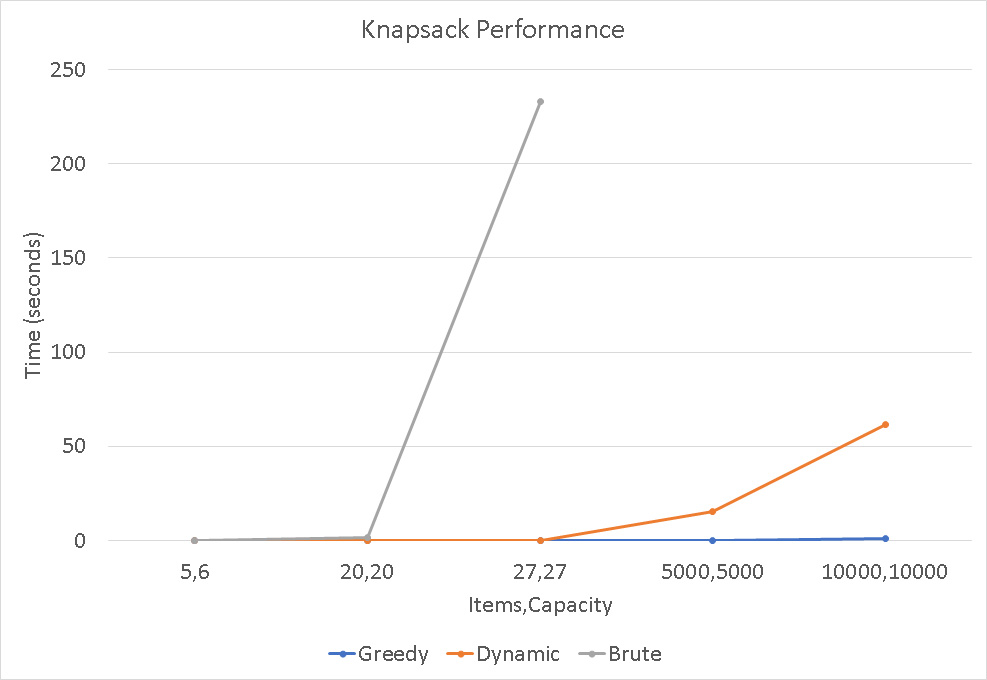
\includegraphics[width=\textwidth]{knapGraph.jpg}
\end{figure}

\newpage
\section{Complexity Analysis}
\subsection{Efficiency per Algorithm}
\begin{table}[H]
    \begin{tabular}{c c c}
        Algorithm & Time & Space \\ \hline
        Greedy & O(n*c), O(n^2) & O(n), O(c) \\ 
        Dynamic & O(n*c) & O(n*c) \\
        Exhaustive & $\Theta$(n!*n) & $\Theta$(n!*n)\\
    \end{tabular}
\end{table}

\subsection{Time Efficiency}
\subsubsection[Greedy Ratio]{Greedy Ratio: O(n*c) or O(n^2)}
\hspace{\parindent}The method needs to iterate through all items (n) to find the one with the best value-to-weight ratio. It keeps looping through this until either the knapsack is full or all items have been added. There is no certainty whether the total weight of all items (n) or the capacity (c) will be the limiting factor for the second dimension. It will be limited by whichever is smaller.

In reality, a situation where the total weight of all items is greater than the knapsack capacity is arguably more likely. So real-world performance scenarios will probably reflect O(n*c).
\subsubsection[Dynamic Programming]{Dynamic Programming: O(n*c)}
\hspace{\parindent}Since the method inherently fills up and utilizes a 2D list, the efficiency will always be limited by the list's dimensions of items (n) by capacity (c).
\subsubsection[Exhaustive Search]{Exhaustive Search: {\boldmath$\Theta$}(n!*n)}
\hspace{\parindent}The brute force method iterates through every possible combination of items from 1 to either number of items (n) or capacity (c). In the worst case, the greatest number of combinations always occurs at nC$\frac{n}{2}$, which scales with n!.

Then for each combination, the algorithm must also iterate through every item within and tally the weight and value. It calculates the combo's total weight to see if it fits in the knapsack, as well as determines if it represents the highest total value. In the worst case of nC$\frac{n}{2}$, the largest combination size thus equals $\frac{n}{2}$, which scales with n.

A best case scenario will occur as long as capacity (c) is less than $\frac{n}{2}$. In this case, efficiency will be $\Omega$(nCc * c).

\subsection{Space Efficiency}
\subsubsection[Greedy Ratio]{Greedy Ratio: O(n) or O(c)}
\hspace{\parindent}The algorithms stores items selected in a list, and refers to the list when selecting subsequent items to avoid redundant selections. Thus, storage scales with either the total weight of all items (n) or capacity (c), whichever is smaller. In real-world scenarios, capacity will likely be the limiting factor.
\subsubsection[Dynamic Programming]{Dynamic Programming: O(n*c)}
\hspace{\parindent}At its core, the method depends on storing previously calculated values in a 2D list, so space efficiency will be the list's dimensions of items (n) by capacity (c).
\subsubsection[Exhaustive Search]{Exhaustive Search: {\boldmath$\Theta$}(n!*n)}
\hspace{\parindent}Since the method iterates through a generated list of combinations, the number of elements stored in memory will peak at nC$\frac{n}{2}$ * $\frac{n}{2}$, which essentially scales with n!*n.

As with time efficiency, the best case will occur when c is less than $\frac{n}{2}$. In this case, space efficiency will be $\Omega$(nCc * c).

\newpage
\section{Schedule}
\begin{table}[H]
    \centering
    \begin{tabular}{c l l}
        Date & Plan & Completed \\ \hline
        4/5 & begin work on program & \\
        4/7 & complete exhaustive search & greedy ratio method\\
        4/9 & complete dynamic programming method & \\
        4/10 & complete third method & exhaustive search method\\
        4/11 & conduct time trials; begin report & dynamic programming method\\
        4/12 & complete program and report & program, time trials\\
        4/13 & & report
    \end{tabular}
\end{table}

\newpage
\section{Screenshot Showcase}
\begin{figure}[H]
    \centering
    \begin{minipage}{0.49\textwidth}
        \centering
        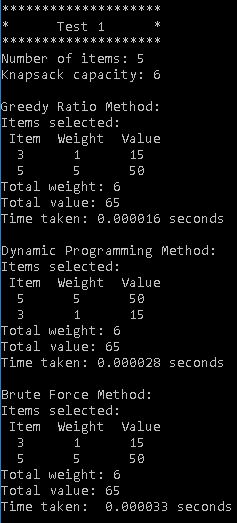
\includegraphics[width=0.95\textwidth]{test1.JPG}
        \caption{Results for 5 items, 6 capacity.}
    \end{minipage}\hfill
    \begin{minipage}{0.49\textwidth}
        \centering
        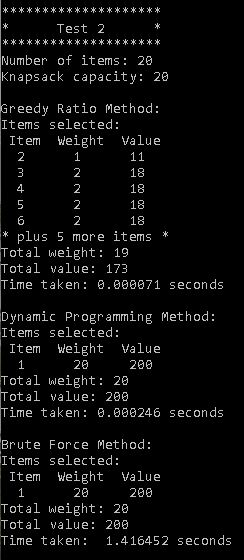
\includegraphics[width=0.95\textwidth]{test2.JPG}
        \caption{Results for 20 items, 20 capacity.}
    \end{minipage}\hfill
\end{figure}
\begin{figure}[H]
    \centering
    \begin{minipage}{0.49\textwidth}
        \centering
        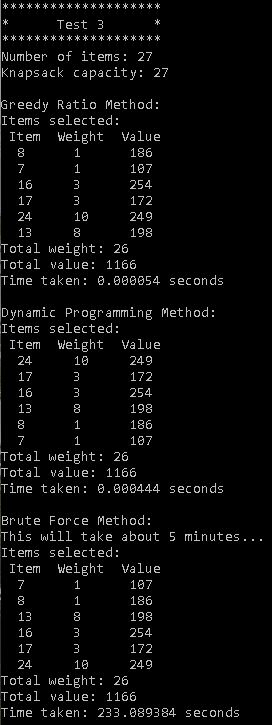
\includegraphics[width=0.95\textwidth]{test3.JPG}
        \caption{Results for 27 items, 27 capacity.}
    \end{minipage}\hfill
    \begin{minipage}{0.49\textwidth}
        \centering
        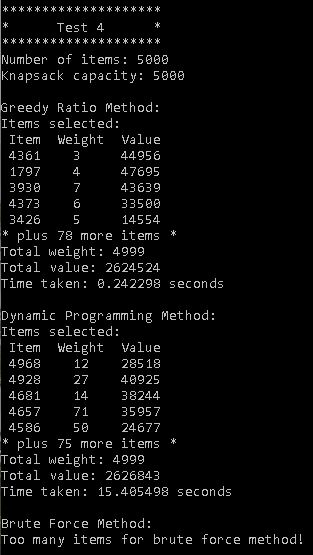
\includegraphics[width=0.95\textwidth]{test4.JPG}
        \caption{Results for 5000 items, 5000 capacity.}
    \end{minipage}\hfill
\end{figure}
\begin{figure}[H]
    \centering
    \begin{minipage}{0.49\textwidth}
        \centering
        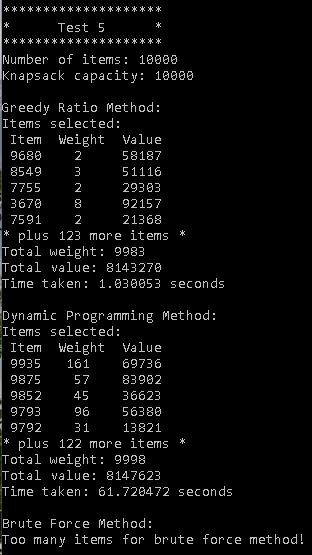
\includegraphics[width=0.95\textwidth]{test5.JPG}
        \caption{Results for 10000 items, 10000 capacity.}
    \end{minipage}\hfill
    \begin{minipage}{0.49\textwidth}
        \centering
        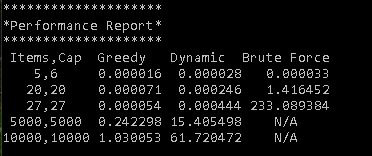
\includegraphics[width=0.95\textwidth]{report.JPG}
        \caption{Performance Report}
    \end{minipage}\hfill
\end{figure}

\end{document}
